% =====================================================================
%  Introduction to Deep Learning — Class 17
%  Topic (course plan): Deep Networks
%  Subtopic (course plan): Revisit Bias-Variance and Double Descent
%  Sources (course plan): Bishop Chapter 9, and Prince Chapter 8
%
%  Classes 13-15 asked how to reach a minimum of the TRAINING error.
%  This class asks what the TEST error is made of, and why the classical
%  answer stops being true for large models.  Order: decompose the error
%  exactly, read the classical trade-off off the decomposition, then the
%  measurement that contradicts it, then the mechanism.
%
%  Nothing here proposes a fix; that is Classes 18 and 19.
%
%  Three results are stated in neither textbook; the C variant is this
%  deck with those three removed.  See _shared/PLAN_Classes17_18_19.md.
%
%  Compile:  xelatex main.tex   (run twice)
% =====================================================================
\documentclass[aspectratio=169, 11pt]{beamer}

\usetheme{metropoliscustom}

\usepackage{graphicx}
\DeclareGraphicsExtensions{.pdf,.png,.jpg}
\graphicspath{{figs/}{Class17_BiasVariance_DoubleDescent/B_Recreated_Figures/figs/}}
\usepackage{amsmath, amssymb}
\usepackage{bm}
\usepackage{tikz}
\usetikzlibrary{arrows.meta, positioning, calc, decorations.pathreplacing,
                shapes.geometric, fit, backgrounds}
\tcbuselibrary{skins}

\definecolor{shc}{HTML}{341651}
\definecolor{tealc}{HTML}{1C7293}
\definecolor{dpc}{HTML}{800000}
\definecolor{accc}{HTML}{B8860B}

% ---- theorem environments -------------------------------------------
\setbeamertemplate{theorems}[numbered]
\usepackage{remreset}
\makeatletter\@removefromreset{theorem}{section}\makeatother
\renewcommand{\thetheorem}{\arabic{theorem}}
\newtheorem{lemmax}[theorem]{Lemma}
\newtheorem{propx}[theorem]{Proposition}
\newtheorem{corx}[theorem]{Corollary}
\newtheorem{defx}[theorem]{Definition}
\newtheorem{thmx}[theorem]{Theorem}

% ---- parallel strip -------------------------------------------------
\newcommand{\twopar}[4]{%
  \vfill
  {\scriptsize
  \begin{tcolorbox}[enhanced, sidebyside, sidebyside align=top,
                    lefthand ratio=0.485,
                    segmentation style={shc!35, line width=0.6pt},
                    colback=shc!5, colframe=shc!35, boxrule=0.5pt,
                    arc=1.2mm, left=1.6mm, right=1.6mm,
                    top=0.6mm, bottom=0.6mm,
                    before skip=0pt, after skip=0pt]
    {\color{shc}\textbf{#1}}\hspace{0.55em}#2
  \tcblower
    {\color{dpc}\textbf{#3}}\hspace{0.55em}#4
  \end{tcolorbox}}%
  \vspace{0.35em}%
}

\newcommand{\bridge}[1]{%
  {\scriptsize\itshape\color{mcMuted} #1\par}\vspace{0.35em}}

\newcommand{\srcline}[1]{%
  \par\vspace{0.25em}%
  {\scriptsize\color{mcMuted}\hfill #1\par}}

\newcommand{\figsource}[1]{{\scriptsize\color{mcMuted} #1}}
\newcommand{\figcap}[2][0.90]{%
  \begin{center}\begin{minipage}{#1\textwidth}\centering
    {\scriptsize\color{mcMuted} #2}
  \end{minipage}\end{center}}

% =====================================================================
\title{Deep Networks}
\subtitle{Bias, Variance and Double Descent}
\author{Introduction to Deep Learning \ \textperiodcentered\ Class 17}
\institute{}
\date{}

\footleft{Introduction to Deep Learning}
\footright{Bias, Variance and Double Descent}
\titlelogos{}

\begin{document}

\maketitle

\begin{frame}{Outline}
  \tableofcontents
\end{frame}

% =====================================================================
\section{What We Are Measuring}
% =====================================================================

\begin{frame}{From training error to test error}
  \bridge{Classes 13 to 15 asked how to reach a minimum of
  $E(\mathbf{w})$ on the training set. Nothing so far has asked what that
  buys on data we have not seen.}
  \vspace{0.35em}
  {\footnotesize
  \renewcommand{\arraystretch}{1.36}
  \begin{tabular}{@{}l@{\hspace{1.6em}}l@{}}
    \textbf{Settled in Classes 13--15} & \textbf{Open today}\\
    how to descend $E(\mathbf{w})$ efficiently & what the error on unseen data
      is made of\\
    how conditioning governs the rate & how that error moves with model size\\
    how to make the landscape kind & why very large models are not ruined\\
  \end{tabular}}
  \vspace{0.9em}

  \begin{redhighlight}
    Today is diagnostic. We decompose the test error exactly, then find
    a measurement the decomposition does not predict.
  \end{redhighlight}
\end{frame}

\begin{frame}{Notation for today}
  \vspace{0.4em}
  {\footnotesize
  \renewcommand{\arraystretch}{1.34}
  \begin{columns}[T, onlytextwidth]
    \begin{column}{0.49\textwidth}
      \begin{tabular}{@{}l@{\hspace{1.5em}}l@{}}
        $\mathcal{D} = \{\mathbf{x}_n, Y_n\}$ & one training set of size $N$\\
        $\hat y(\mathbf{x}; \mathcal{D})$ & the model fitted to that set\\
        $h(\mathbf{x}) = \mathbb{E}[Y \,|\, \mathbf{x}]$ & the regression function\\
        $\sigma^2$ & variance of $Y$ about $h(\mathbf{x})$\\
      \end{tabular}
    \end{column}
    \begin{column}{0.49\textwidth}
      \begin{tabular}{@{}l@{\hspace{1.5em}}l@{}}
        $\mathbb{E}_{\mathcal{D}}[\cdot]$ & average over training sets\\
        $\bar y(\mathbf{x})$ & $\mathbb{E}_{\mathcal{D}}[\hat y(\mathbf{x};\mathcal{D})]$, the ensemble mean\\
        $p$ & number of learnable parameters\\
        $\gamma = p/N$ & parameters per observation\\
      \end{tabular}
    \end{column}
  \end{columns}}
  \vspace{0.7em}

  \begin{itemize}\itemsep0.3em
    \item Bishop writes $h(\mathbf{x})$ and Prince writes $\mu[\mathbf{x}]$ for
          the same object; both mean the conditional mean of the target
  \end{itemize}
  \srcline{Bishop \& Bishop (2024), Eq.~4.41; Prince (2023), Eq.~8.1.}
\end{frame}

\begin{frame}{Three data sets, three different objectives}
  \vspace{-0.1em}
  \begin{center}
  \begin{tikzpicture}[>=Stealth, font=\scriptsize, scale=0.98,
      box/.style={rounded corners=2pt, draw, line width=1.0pt,
                  minimum height=1.05cm, align=center, inner sep=4pt},
      lbl/.style={align=center, font=\scriptsize}]
    \node[box, fill=shc!12,   draw=shc,   text width=3.5cm] (tr) at (0,0)
      {\textbf{training set}\\ fit $\mathbf{w}$};
    \node[box, fill=tealc!12, draw=tealc, text width=3.5cm] (va) at (4.5,0)
      {\textbf{validation set}\\ choose hyperparameters};
    \node[box, fill=dpc!12,   draw=dpc,   text width=3.5cm] (te) at (9.0,0)
      {\textbf{test set}\\ report performance};

    \draw[->, shc,   line width=1.2pt] (tr) -- (va);
    \draw[->, tealc, line width=1.2pt] (va) -- (te);

    \node[lbl, shc,   below=3pt of tr] {gradient descent\\ touches this};
    \node[lbl, tealc, below=3pt of va] {model selection\\ touches this};
    \node[lbl, dpc,   below=3pt of te] {nothing may\\ touch this};
  \end{tikzpicture}
  \end{center}
  \vspace{0.2em}
  \begin{itemize}\itemsep0.3em
    \item Hyperparameters chosen on the test set would report a number
          that cannot be reproduced on new data
    \item The hyperparameter space is discrete and conditional, so
          gradient descent cannot search it
  \end{itemize}
  \srcline{Prince (2023), \S8.5.}
\end{frame}

% =====================================================================
\section{The Decomposition}
% =====================================================================

\begin{frame}{The best predictor there is}
  \vspace{-0.2em}
  \begin{propx}[The conditional mean minimises squared loss]\label{th:cond}
    \small
    \vspace{-0.2em}
    For squared loss the expected loss of any function $f$ splits as
    \[
      \mathbb{E}[L] = \int \{f(\mathbf{x}) - h(\mathbf{x})\}^2 \, p(\mathbf{x})\,\mathrm{d}\mathbf{x}
        \;+\; \int \mathrm{var}[Y \,|\, \mathbf{x}]\, p(\mathbf{x})\,\mathrm{d}\mathbf{x},
    \]
    so it is minimised by $f = h$, and the second term does not depend
    on $f$ at all.
  \end{propx}
  \vspace{0.05em}
  \begin{itemize}\itemsep0.24em
    \item The second term is the \alert{noise}: the price of predicting
          a random variable with a function
    \item No model, no data set and no algorithm can reduce it
    \item Everything today concerns the first term
  \end{itemize}
  \srcline{Bishop \& Bishop (2024), Eqs.~4.39, 4.42.}
\end{frame}

\begin{frame}{Where the error comes from}
  \begin{center}
    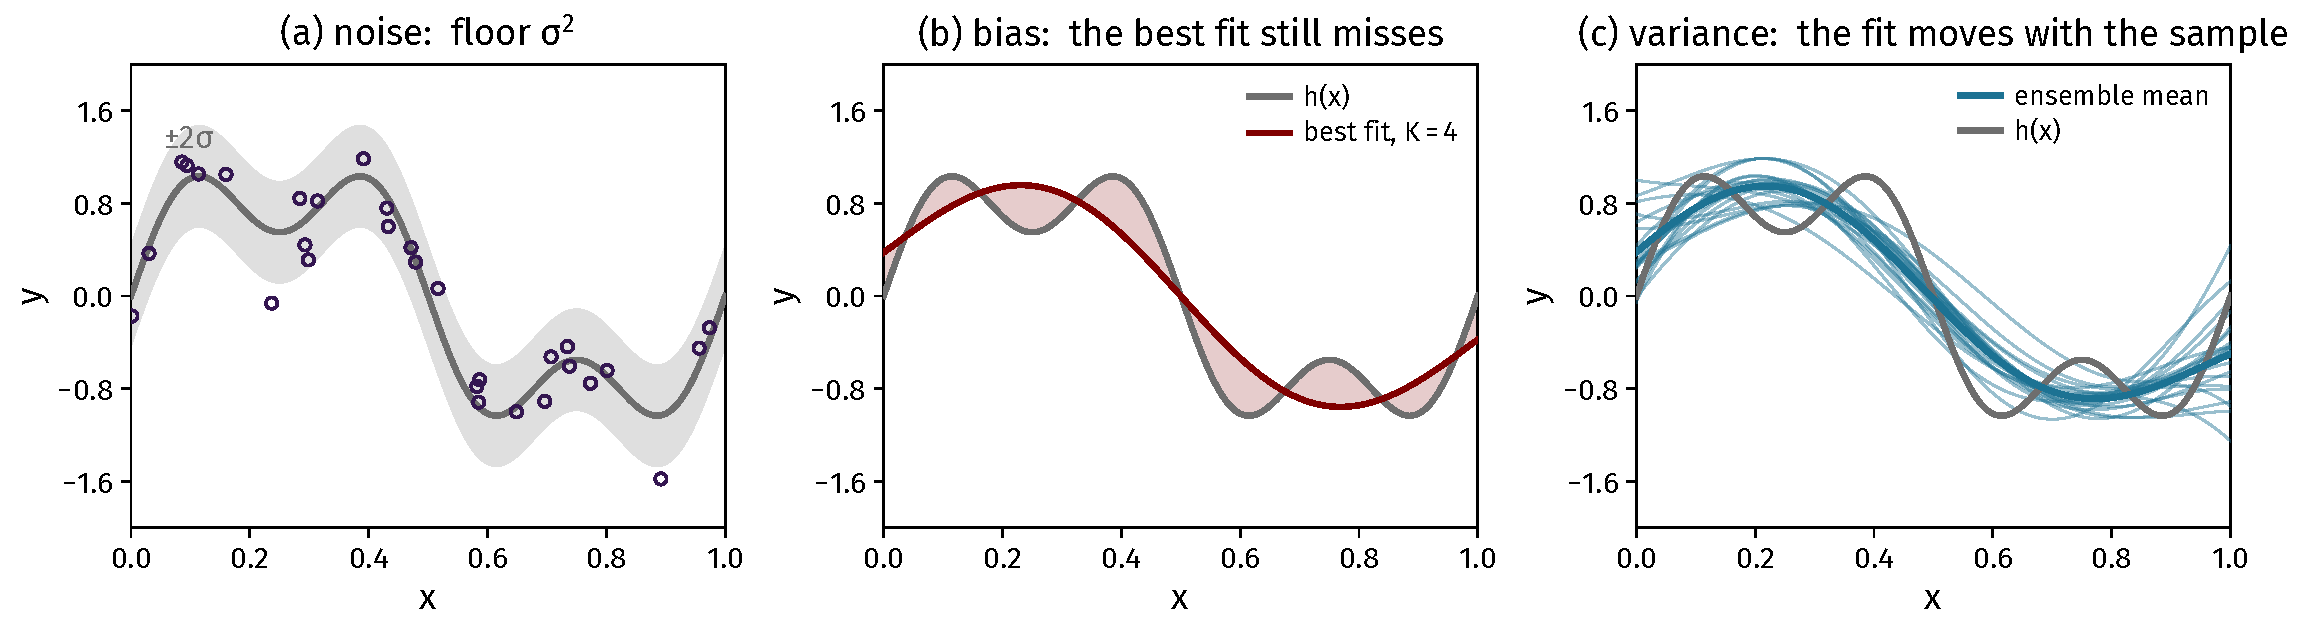
\includegraphics[width=0.97\linewidth]{error_sources}
  \end{center}
  \figcap[0.97]{(a) the targets scatter about $h(x)$, so a floor
  $\sigma^2$ remains however good the model. (b) a model of limited
  capacity misses $h(x)$ even when fitted to infinite noiseless data.
  (c) fitted to a finite noisy sample it misses again, differently each
  time.}
\end{frame}

\begin{frame}{The decomposition}
  \vspace{-0.25em}
  \begin{thmx}[Bias--variance--noise]\label{th:decomp}
    \small
    For squared loss, at each $\mathbf{x}$,
    \[
      \underbrace{\mathbb{E}_{\mathcal{D}}\,\mathbb{E}_{Y}\big[(\hat y(\mathbf{x};\mathcal{D}) - Y)^2\big]}_{\text{expected test error}}
      =
      \underbrace{\mathbb{E}_{\mathcal{D}}\big[(\hat y(\mathbf{x};\mathcal{D}) - \bar y(\mathbf{x}))^2\big]}_{\text{variance}}
      +
      \underbrace{(\bar y(\mathbf{x}) - h(\mathbf{x}))^2}_{\text{bias}^2}
      +
      \underbrace{\sigma^2}_{\text{noise}} .
    \]
  \end{thmx}
  \vspace{0.1em}
  {\footnotesize
  \begin{itemize}\itemsep0.24em
    \item \alert{Bias} is how far the \emph{average} model is from the
          truth --- a property of the model class
    \item \alert{Variance} is how far a \emph{single} model is from that
          average --- a property of the sample
    \item The three terms are additive here; for other losses they
          interact
  \end{itemize}}
  \srcline{Prince (2023), Eq.~8.7; Bishop \& Bishop (2024), Eqs.~4.45--4.49.}
\end{frame}

\begin{frame}{Proof, in two identical steps}
  \vspace{-0.3em}
  {\footnotesize
  \begin{itemize}\itemsep0.30em
    \item \focus{1}{Add and subtract $h(\mathbf{x})$ inside the square:
          $(\hat y - Y)^2 = \{(\hat y - h) + (h - Y)\}^2$.}
    \item \focus{2}{Expanding gives a cross term
          $2(\hat y - h)(h - Y)$, whose expectation over $Y$ vanishes
          because $\mathbb{E}_Y[Y] = h(\mathbf{x})$ by definition.}
    \item \focus{3}{What survives is
          $\mathbb{E}_Y[(\hat y - Y)^2] = (\hat y - h)^2 + \sigma^2$.
          The noise has separated.}
    \item \focus{4}{Now repeat the same move on $(\hat y - h)^2$,
          this time adding and subtracting $\bar y(\mathbf{x})$ and
          averaging over $\mathcal{D}$.}
    \item \focus{5}{The cross term $2(\hat y - \bar y)(\bar y - h)$
          vanishes for the same reason: $\mathbb{E}_{\mathcal{D}}[\hat y] = \bar y$
          by definition.}
    \item \focus{6}{This leaves variance $+$ bias$^2$, and with the
          $\sigma^2$ from step 3 the theorem follows. \hfill $\square$}
  \end{itemize}}
  \vspace{-0.15em}
  \begin{redhighlight}
    One algebraic move, used twice: add and subtract the mean, and the
    cross term dies because a deviation from a mean has zero mean.
  \end{redhighlight}
\end{frame}

\begin{frame}{What the decomposition is and is not}
  \vspace{0.15em}
  \begin{corx}[The floor]\label{th:floor}
    \small
    Since variance $\geq 0$ and bias$^2 \geq 0$, the expected test error
    is at least $\sigma^2$, with equality only if the fitted model
    equals $h$ for every training set.
  \end{corx}
  \vspace{0.25em}
  \begin{itemize}\itemsep0.3em
    \item Both terms are averages over an \alert{ensemble} of training
          sets; in practice we hold exactly one
    \item So neither term is measurable from the data we have, which is
          why validation exists
    \item Given several independent training sets one would combine
          them rather than average over them
  \end{itemize}
  \srcline{Bishop \& Bishop (2024), \S4.3; Prince (2023), \S8.2.2.}
\end{frame}

% =====================================================================
\section{The Classical Trade-off}
% =====================================================================

\begin{frame}{Two ways to spend capacity}
  \begin{center}
    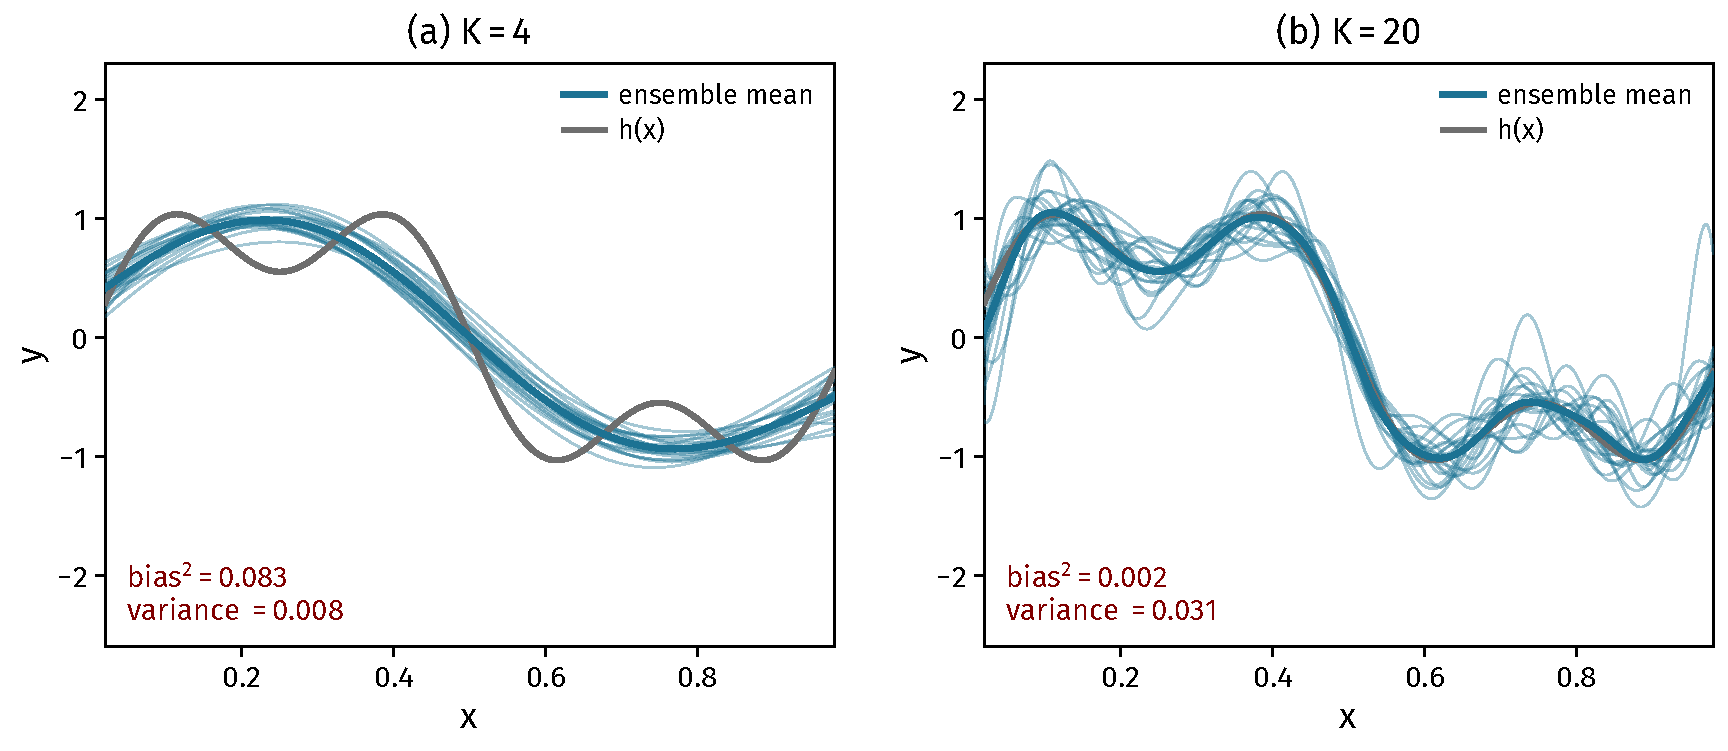
\includegraphics[width=0.78\linewidth]{capacity_fits}
  \end{center}
  \figcap[0.97]{Twenty fits, each to its own sample of $N = 60$ points.
  (a) the fits agree with each other and disagree with $h(x)$.
  (b) they disagree with each other and their mean agrees with $h(x)$.}
\end{frame}

\begin{frame}{The trade-off, measured}
  \begin{center}
    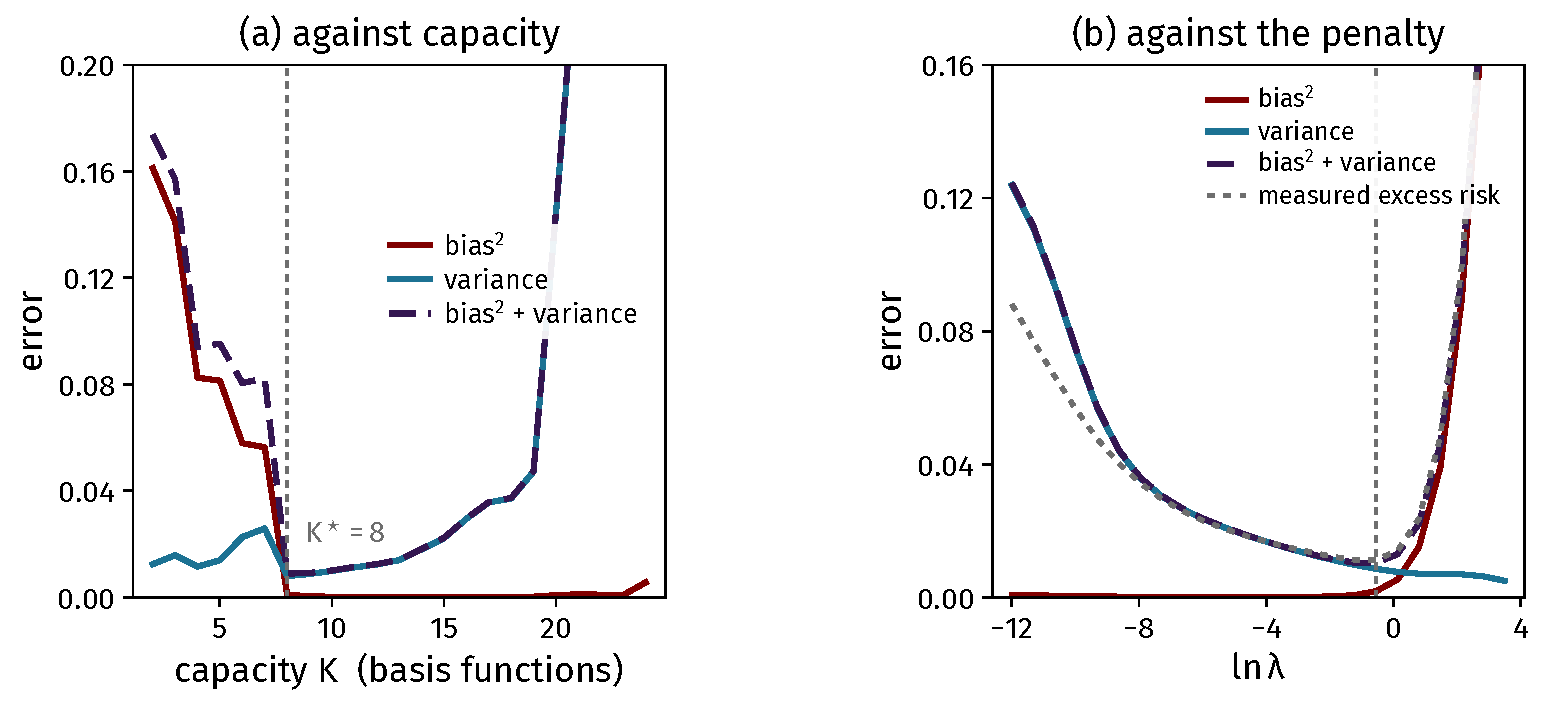
\includegraphics[width=0.78\linewidth]{tradeoff_curve}
  \end{center}
  \figcap[0.97]{Both terms by Monte Carlo over $200$ training sets.
  (a) against capacity: the sum is smallest at $K^\star = 8$.
  (b) against the penalty: the measured excess risk lies on top of
  bias$^2 +$ variance, as the theorem requires.}
\end{frame}

\begin{frame}{What reduces each term}
  \vspace{0.3em}
  {\footnotesize
  \renewcommand{\arraystretch}{1.42}
  \begin{tabular}{@{}l@{\hspace{1.3em}}l@{\hspace{1.3em}}l@{}}
    \textbf{Term} & \textbf{Reduced by} & \textbf{At the cost of}\\
    noise $\sigma^2$ & nothing & ---\\
    bias$^2$ & more capacity & more variance\\
    variance & more data & data is what is scarce\\
    variance & a penalty on $\mathbf{w}$ & more bias\\
  \end{tabular}}
  \vspace{0.7em}

  \begin{itemize}\itemsep0.3em
    \item More data lowers variance without raising bias, which is why
          it is the one intervention with no trade
    \item Every other row is a trade, and the classical conclusion is
          that some interior capacity is best
  \end{itemize}
  \srcline{Prince (2023), \S8.3.1--8.3.3.}
\end{frame}

\begin{frame}{The classical prescription}
  \vspace{0.2em}
  \begin{block}{The received view}
    \small
    Test error is U-shaped in model complexity. Choose the model whose
    capacity matches the size of the data set: too small and bias
    dominates, too large and variance dominates. Very large models
    trained on modest data sets are therefore expected to generalize
    badly.
  \end{block}
  \vspace{0.1em}
  \begin{itemize}\itemsep0.24em
    \item A correct reading of the decomposition, and of every curve on
          the previous slide
    \item It is also the standard advice in classical statistics
    \item Modern networks have far more parameters than training points
  \end{itemize}
  \srcline{Bishop \& Bishop (2024), \S9.3.2.}
\end{frame}

% =====================================================================
\section{Double Descent}
% =====================================================================

\begin{frame}{What is actually measured}
  \begin{center}
    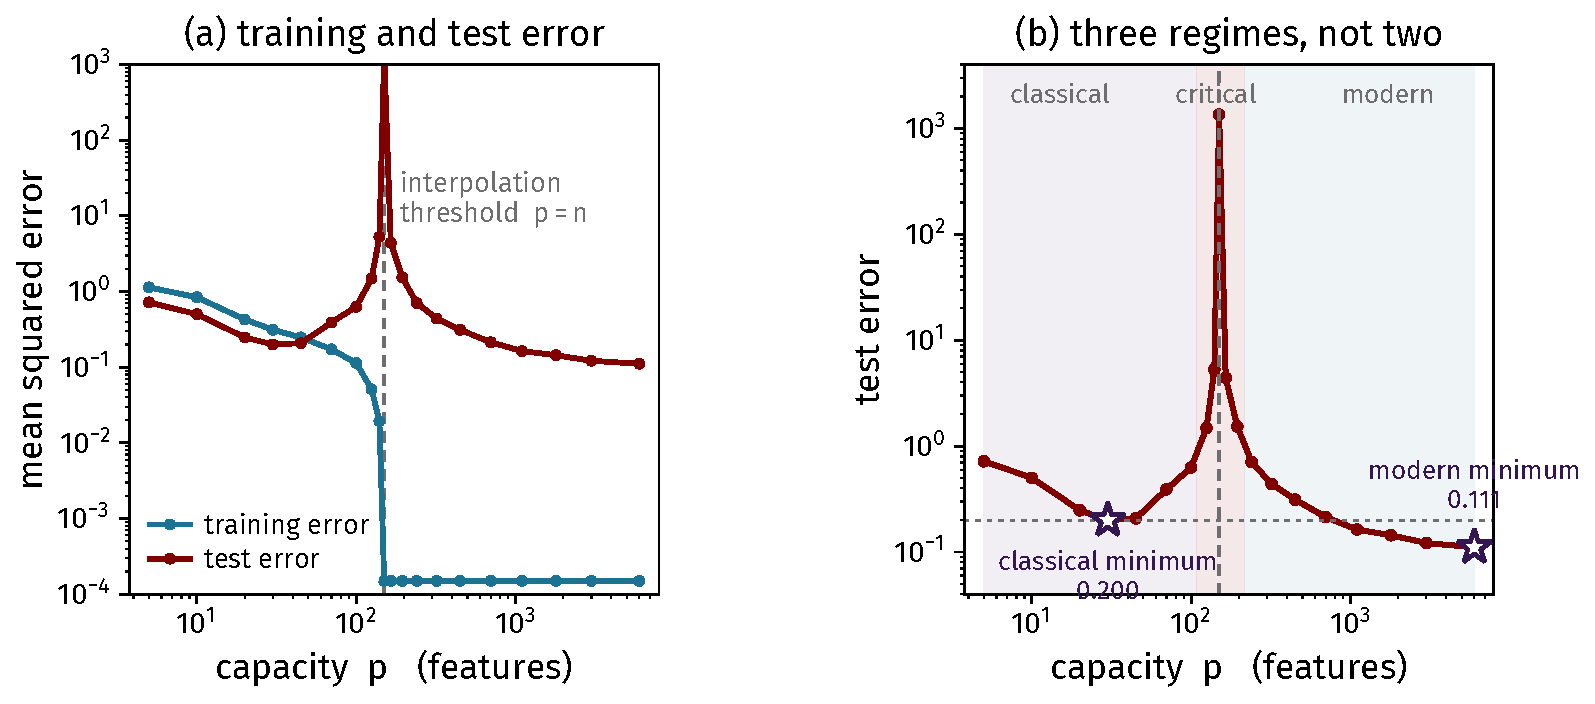
\includegraphics[width=0.78\linewidth]{double_descent}
  \end{center}
  \figcap[0.97]{$N = 150$ points, $p$ random features, minimum-norm
  least squares, no penalty and no stopping. (a) training error reaches
  zero at $p = N$. (b) test error peaks there, then descends below its
  classical best.}
\end{frame}

\begin{frame}{The same curve, in the ResNet layout}
  \begin{center}
    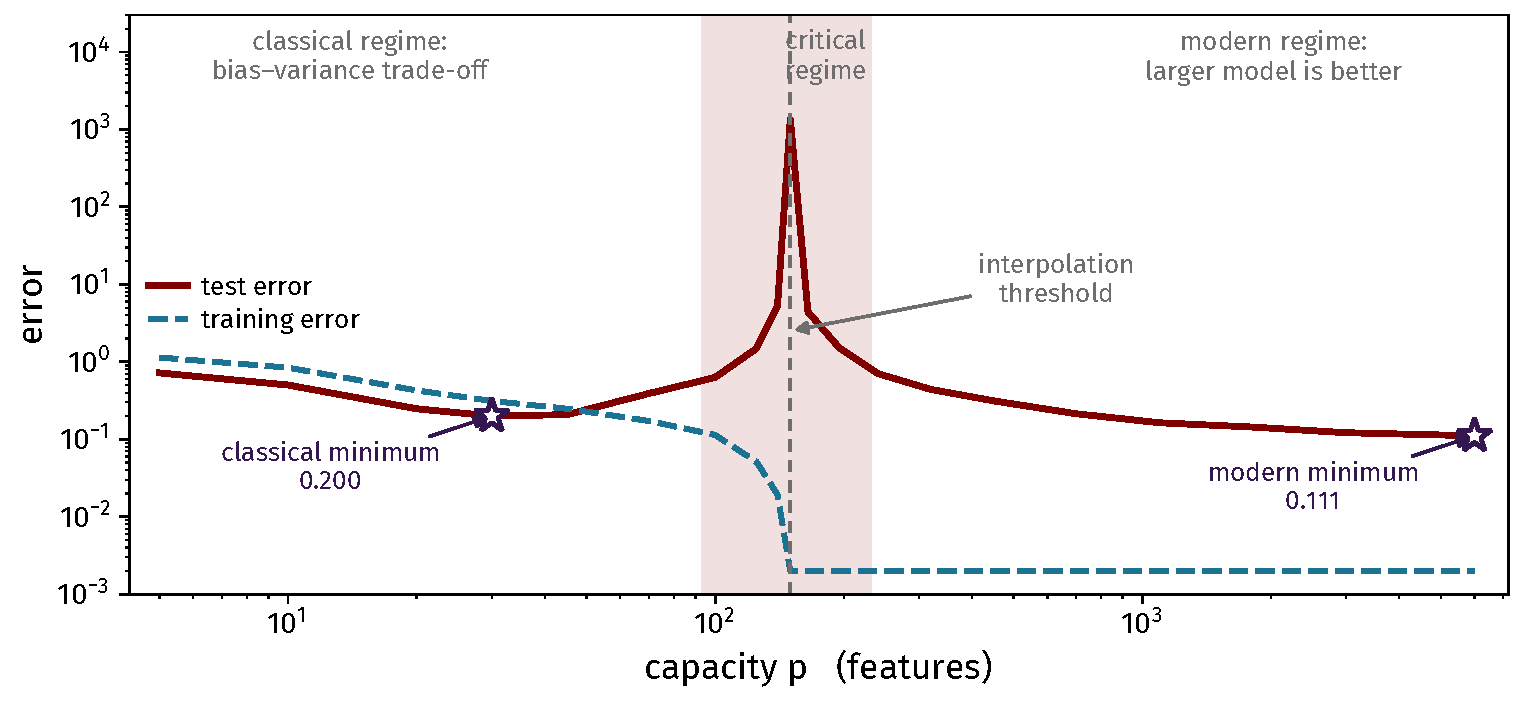
\includegraphics[height=0.50\textheight]{double_descent_regimes}
  \end{center}
  \figcap[0.97]{The previous experiment drawn as the ResNet18 result is:
  both errors on one axis, the critical regime shaded, the threshold
  marked.}
\end{frame}

\begin{frame}{Reading the curve}
  \vspace{0.1em}
  {\footnotesize
  \begin{itemize}\itemsep0.34em
    \item \textbf{Axes.} Capacity $p$ is the number of parameters;
          $N = 150$ throughout. Dashed is training error, solid is error
          on unseen data, and only the solid one matters
    \item \textbf{Threshold, $p = N$.} The model can fit every training
          point exactly; the training error reaches zero and stays there
    \item \textbf{Classical regime, $p < N$.} Test error falls as bias
          falls, then rises as variance rises: the U-curve, with its
          \alert{classical minimum} at $0.200$
    \item \textbf{Critical regime, $p \approx N$.} Exactly one interpolant
          exists and it is enormous; the test error peaks three orders of
          magnitude above the minimum
    \item \textbf{Modern regime, $p > N$.} Many interpolants exist and the
          smallest is chosen. Test error descends again to the
          \alert{modern minimum} at $0.111$ --- below the classical one,
          although the training error has been zero since the threshold
  \end{itemize}}
\end{frame}

\begin{frame}{The same shape at four noise levels}
  \begin{center}
    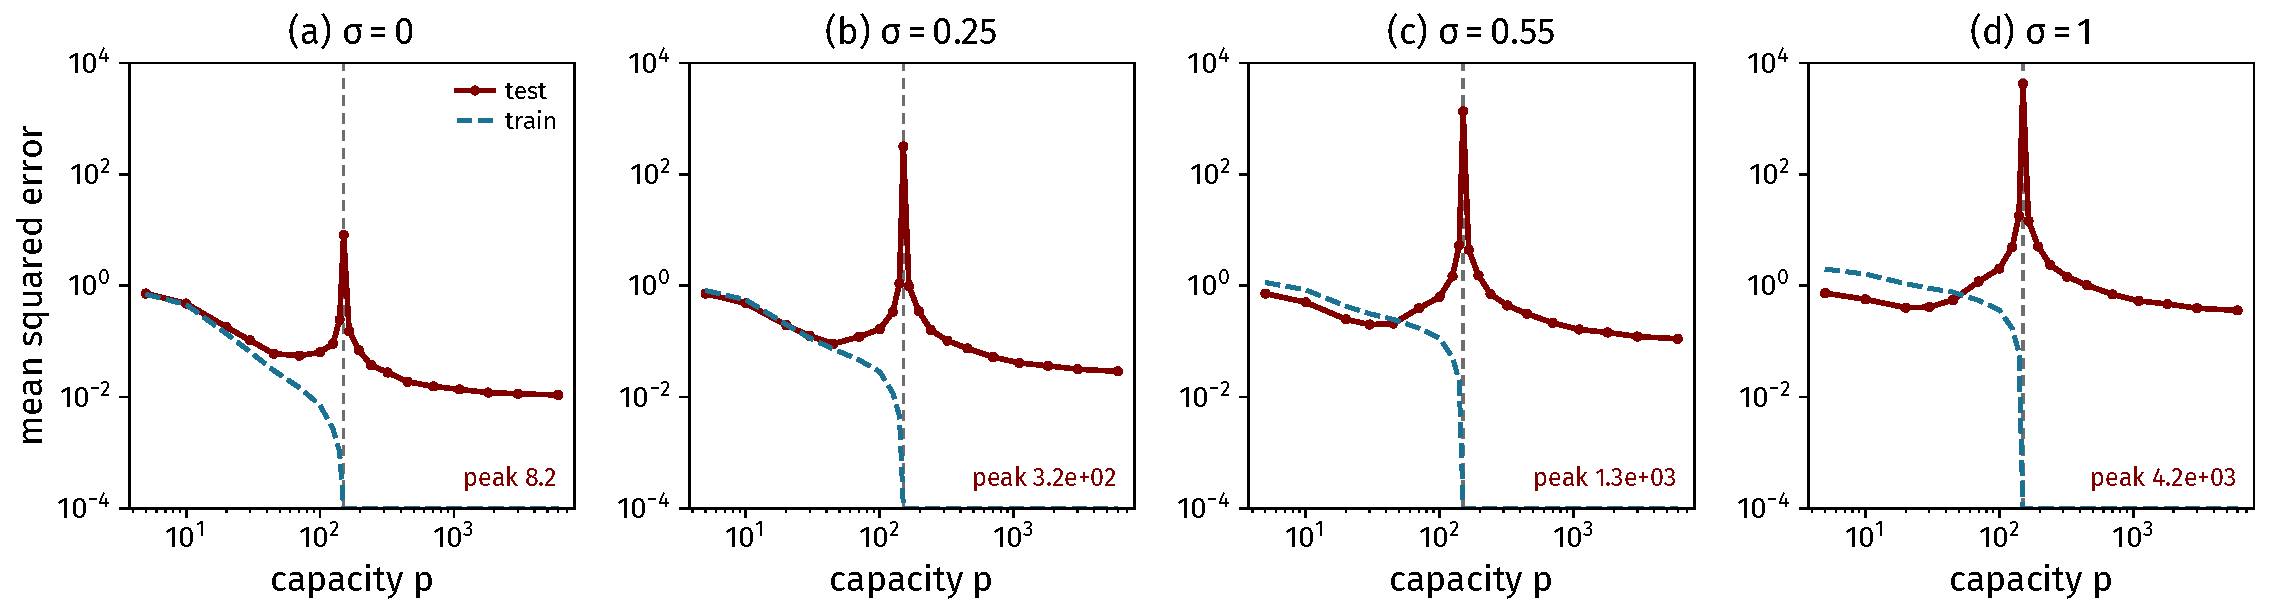
\includegraphics[width=0.96\linewidth]{double_descent_noise}
  \end{center}
  \figcap[0.97]{The same experiment with the label noise set to four
  values and nothing else changed. With clean labels there is barely a
  peak and no classical minimum worth the name; as the noise grows the
  peak grows with it, from $8$ to over $4{,}000$, because at the
  threshold the model must interpolate the noise exactly.}
\end{frame}

\begin{frame}{The interpolation threshold}
  \vspace{-0.1em}
  \begin{defx}[Interpolation threshold]\label{th:thresh}
    \small
    The capacity at which the model first attains zero training error.
    Below it the data constrain the fit; above it a family of exact fits
    exists and the algorithm chooses among them.
  \end{defx}
  \vspace{0.2em}
  \begin{defx}[Effective model complexity]\label{th:emc}
    \small
    The largest training set size on which a given training procedure
    reaches approximately zero training error. Double descent appears
    where it crosses $N$.
  \end{defx}
  \vspace{0.15em}
  \begin{itemize}\itemsep0.25em
    \item Defined for the \alert{procedure}, not the architecture: the
          optimiser and the epoch count are part of it
  \end{itemize}
  \srcline{Belkin et al.\ (2019); Nakkiran et al.\ (2019).}
\end{frame}

\begin{frame}{The risk, in closed form}
  \vspace{-0.25em}
  \begin{thmx}[Ridgeless least squares, isotropic design]\label{th:ridgeless}
    \small
    Let $Y = \mathbf{X}\mathbf{w} + \varepsilon$ with rows of $\mathbf{X}$ drawn from
    $\mathcal{N}(\mathbf{0}, \mathbf{I}_p)$ and $\varepsilon \sim \mathcal{N}(0, \sigma^2)$,
    and let $\hat{\mathbf{w}}$ be the minimum-norm least-squares solution.
    As $N, p \to \infty$ with $p/N \to \gamma$, the excess risk tends to
    \[
      R(\gamma) =
      \begin{cases}
        \dfrac{\sigma^2 \gamma}{1 - \gamma}, & \gamma < 1,\\[0.9em]
        \|\mathbf{w}\|^2\Big(1 - \dfrac{1}{\gamma}\Big)
          + \dfrac{\sigma^2}{\gamma - 1}, & \gamma > 1 .
      \end{cases}
    \]
  \end{thmx}
  \vspace{0.25em}
  \begin{itemize}\itemsep0.25em
    \item Both branches diverge as $\gamma \to 1$: the peak is a pole,
          not an accident of any particular experiment
  \end{itemize}
  \srcline{Hastie, Montanari, Rosset \& Tibshirani (2022), Thm.~1.}
\end{frame}

\begin{frame}{Reading the two branches}
  \vspace{-0.2em}
  {\scriptsize
  \begin{itemize}\itemsep0.30em
    \item \focus{1}{Below the threshold there is one least-squares
          solution and it must absorb the noise in $N - p$ fewer degrees
          of freedom than it has observations; the risk
          $\sigma^2\gamma/(1-\gamma)$ grows as that slack disappears.}
    \item \focus{2}{At $\gamma = 1$ the design is square and almost
          singular. Exactly one vector interpolates, and it is forced to
          be enormous.}
    \item \focus{3}{Above the threshold the interpolating set is an
          affine subspace of dimension $p - N$, and minimum norm picks
          one point of it.}
    \item \focus{4}{Growing $\gamma$ enlarges that subspace, so the
          chosen point can be smaller: the noise term
          $\sigma^2/(\gamma-1)$ falls.}
    \item \focus{5}{The price is the bias term
          $\|\mathbf{w}\|^2(1 - 1/\gamma)$, which rises to $\|\mathbf{w}\|^2$.
          The second descent is the race between the two.}
  \end{itemize}}
  \vspace{-0.2em}
  \begin{redhighlight}
    Two solutions fit the data equally well; the risk depends entirely
    on which of them the algorithm returns.
  \end{redhighlight}
\end{frame}

\begin{frame}{Theory against measurement}
  \begin{center}
    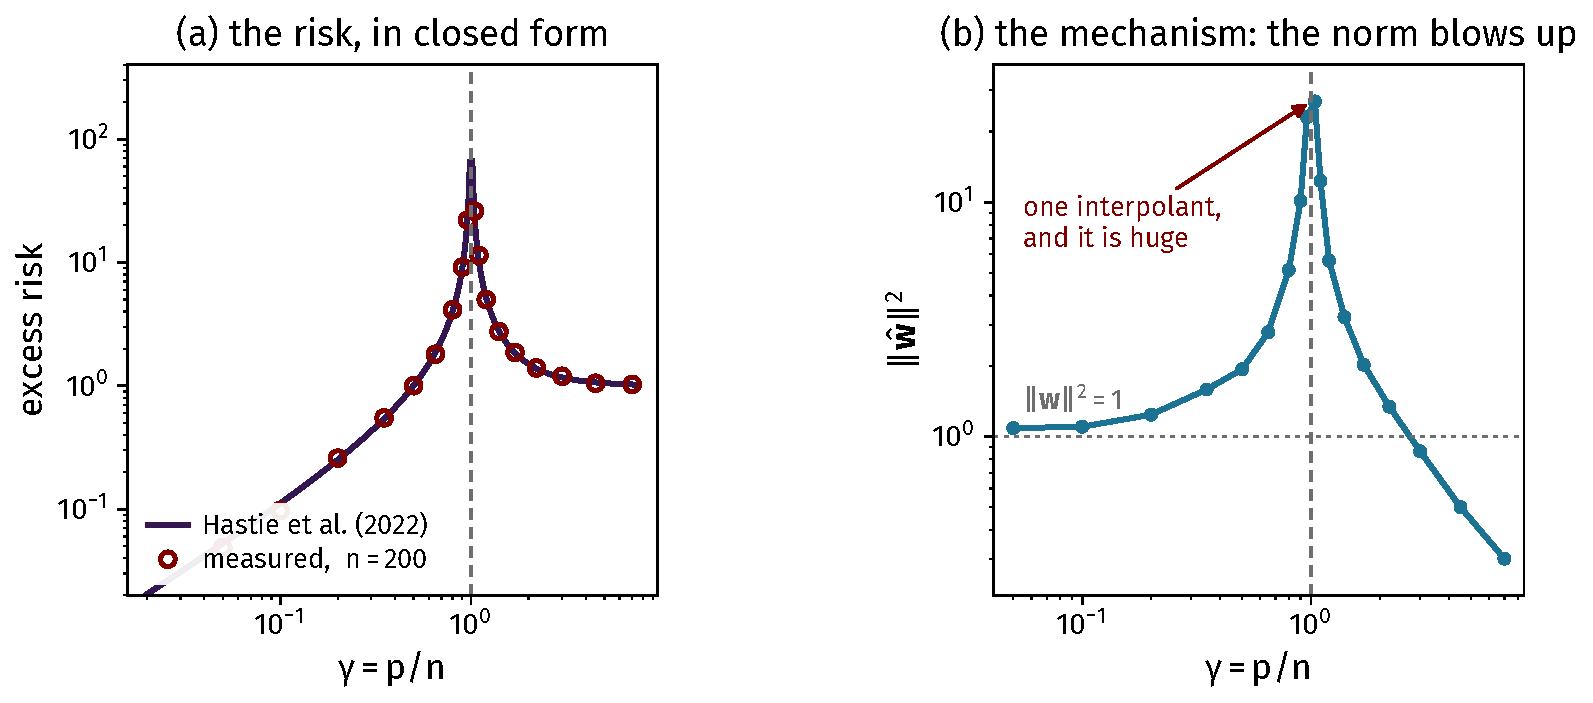
\includegraphics[width=0.78\linewidth]{minnorm_theory}
  \end{center}
  \figcap[0.97]{(a) the closed form against simulation at $n = 200$,
  over four decades and on both sides of the pole. (b) the squared norm
  of the fitted vector, which peaks at exactly the same place.}
\end{frame}

\begin{frame}{Smoothness is what extra capacity buys}
  \begin{center}
    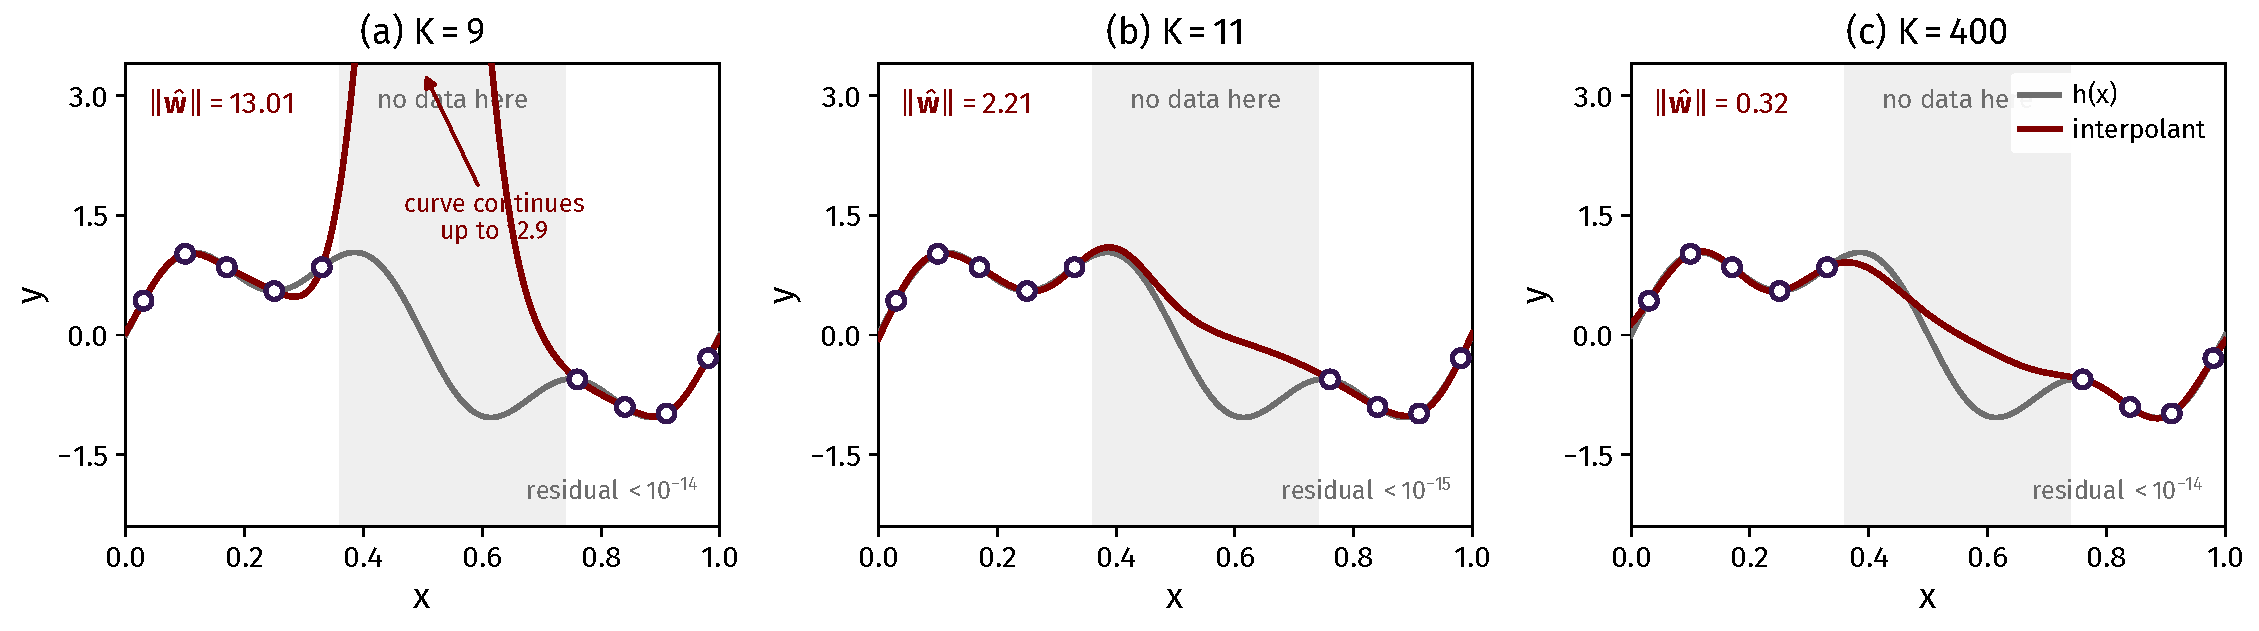
\includegraphics[width=0.97\linewidth]{smooth_interpolants}
  \end{center}
  \figcap[0.97]{Nine points with a gap, fitted exactly in a basis of $K$
  bumps of fixed width; every panel has a training residual below
  $10^{-14}$. With just enough capacity the interpolant leaves the frame
  and climbs to $12.9$ in the gap --- that excursion is the point. As
  $K$ grows it becomes tamer, and $\|\hat{\mathbf{w}}\|$ falls from
  $13.0$ to $0.32$.}
\end{frame}

\begin{frame}{Why sparse data makes this matter}
  \vspace{-0.1em}
  \begin{itemize}\itemsep0.3em
    \item Past the threshold the data are fitted exactly, so extra
          capacity can only change the model \alert{between} the
          training points
    \item In high dimensions almost everything is between them:
          quantising $40$ inputs into $10$ bins gives $10^{40}$ cells for
          $10^{5}$ examples
    \item So what decides the test error is behaviour no training point
          constrains
    \item A procedure's tendency to prefer one such completion is its
          \alert{inductive bias}; here, a preference for small norm and
          so for smoothness
  \end{itemize}
  \bridge{What produces that preference, and how to install one
  deliberately, is the subject of Class 18.}
  \srcline{Prince (2023), \S8.4.1.}
\end{frame}

\begin{frame}{Capacity is not the parameter count}
  \begin{center}
    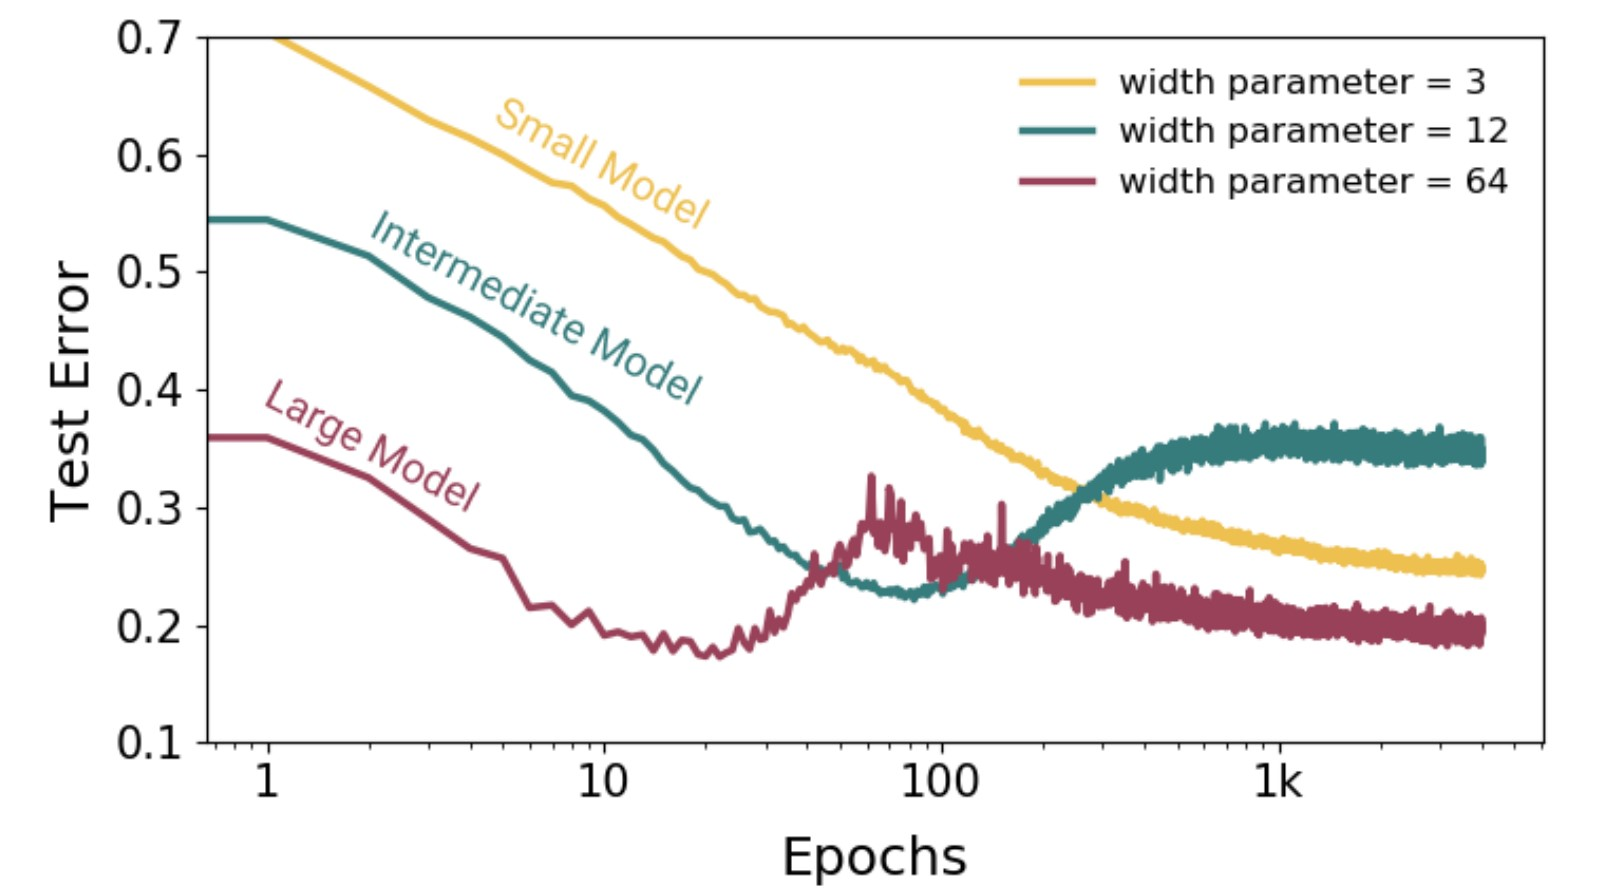
\includegraphics[height=0.48\textheight]{Bishop9_10}
  \end{center}
  \figcap[0.97]{Test error against training epochs for three model
  sizes. Effective complexity grows with the epochs, so the large model
  traverses in time the three regimes the previous figures traversed in
  width: down, up at the threshold, and down again.
  Bishop \& Bishop (2024), Fig.~9.10, from Nakkiran et al.\ (2019).}
\end{frame}

\begin{frame}{The same curve along three different axes}
  \vspace{0.3em}
  {\footnotesize
  \renewcommand{\arraystretch}{1.42}
  \begin{tabular}{@{}l@{\hspace{1.2em}}l@{\hspace{1.2em}}l@{}}
    \textbf{Axis varied} & \textbf{Peak sits at} & \textbf{Name}\\
    number of parameters, $N$ fixed & $p = N$ & model-wise\\
    training epochs, $p$ and $N$ fixed & $d_{\mathrm{eff}} \approx N$ & epoch-wise\\
    training set size, $p$ fixed & $N = p$ & sample-wise\\
    inverse penalty $1/\lambda$ & where the fit first interpolates & ---\\
  \end{tabular}}
  \vspace{0.55em}

  \begin{itemize}\itemsep0.26em
    \item All four are the same statement about effective complexity
          crossing the amount of data
    \item Epoch-wise is why a large model can look worse after longer
          training and better again after longer still
  \end{itemize}
  \srcline{Nakkiran et al.\ (2019); Yilmaz \& Heckel (2022).}
\end{frame}

\begin{frame}{More data can make a model worse}
  \begin{center}
    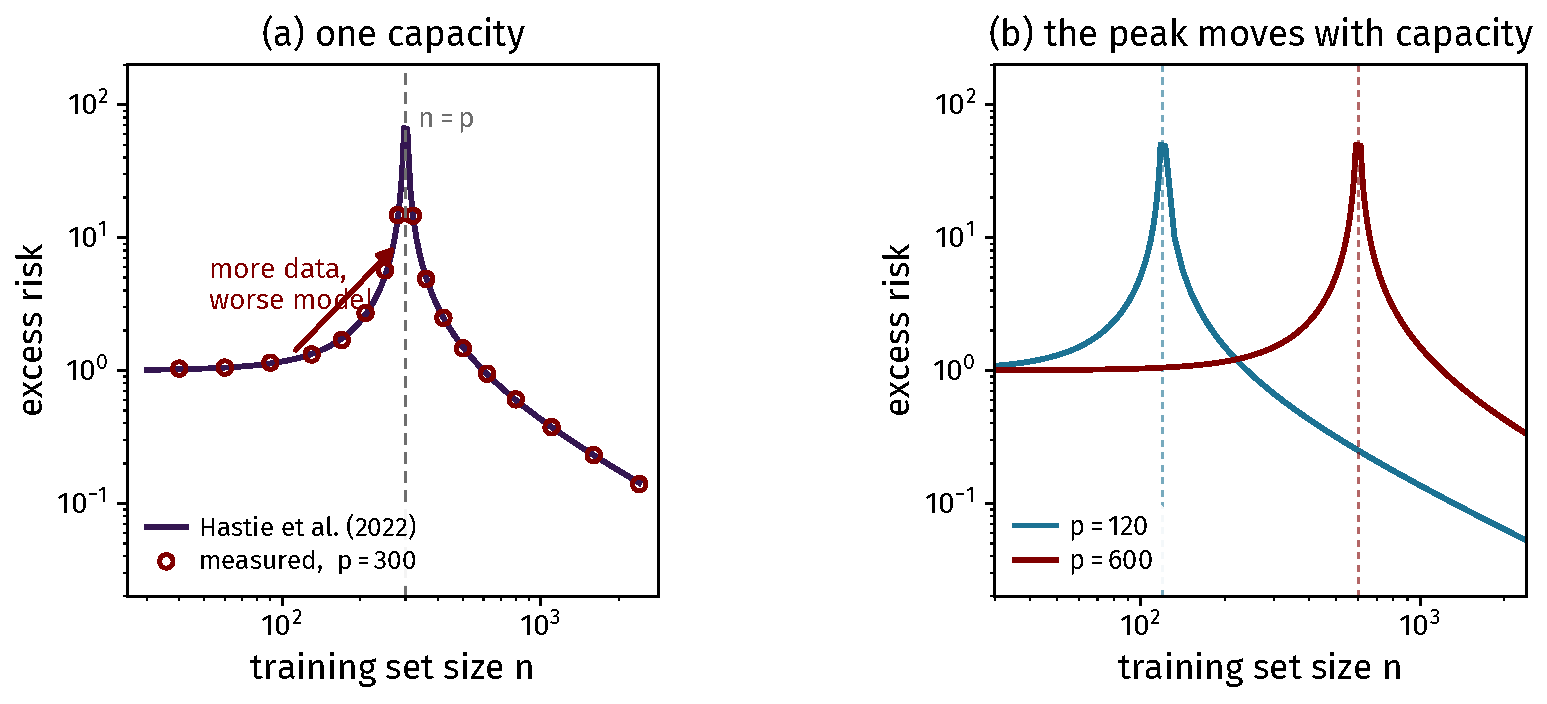
\includegraphics[width=0.78\linewidth]{sample_wise}
  \end{center}
  \figcap[0.97]{Capacity fixed, sample size varied. (a) between
  $N = 100$ and $N = p = 300$ the risk rises: more data is worse there.
  (b) each capacity carries its own peak at its own $N = p$.}
\end{frame}

% =====================================================================
\section{What This Changes}
% =====================================================================

\begin{frame}{What survives and what does not}
  \vspace{0.15em}
  {\scriptsize
  \renewcommand{\arraystretch}{1.40}
  \begin{tabular}{@{}l@{\hspace{1.1em}}l@{}}
    \textbf{Claim} & \textbf{Status}\\
    error $=$ bias$^2$ $+$ variance $+$ noise & exact, and unaffected\\
    noise is irreducible & exact, and unaffected\\
    bias falls with capacity & holds\\
    variance rises with capacity & holds \emph{below} the threshold only\\
    test error is U-shaped in capacity & \alert{false} past the threshold\\
    a model with $p > N$ must over-fit & \alert{false}\\
    more data cannot hurt & \alert{false} near $N = p$\\
  \end{tabular}}
  \vspace{0.6em}

  \begin{redhighlight}
    The decomposition is a theorem and stays true. What fails is the
    empirical claim about how variance behaves once the model can
    interpolate.
  \end{redhighlight}
\end{frame}

\begin{frame}{Choosing capacity when the curve has two minima}
  \vspace{-0.2em}
  \begin{itemize}\itemsep0.28em
    \item Neither term is measurable from one training set, so capacity
          is chosen by \alert{validation}, not by theory
    \item In the classical regime the validation curve has an interior
          minimum, and the search is a line search
    \item In the modern regime it falls with capacity as far as one can
          afford, and the binding constraint becomes compute
    \item The regime to avoid is the critical one, $p \approx N$
  \end{itemize}
  \vspace{0.2em}
  \begin{redhighlight}
    Either stay well below the threshold or go well past it. Sitting on
    it is the one choice the measurements rule out.
  \end{redhighlight}
  \srcline{Prince (2023), \S8.5; Nakkiran et al.\ (2019).}
\end{frame}

\begin{frame}{Takeaways}
  \vspace{0.1em}
  {\scriptsize
  \begin{enumerate}\itemsep0.34em
    \item For squared loss the expected test error is exactly
          bias$^2 +$ variance $+$ noise, and the proof is one algebraic
          move used twice (Theorem~\ref{th:decomp})
    \item Noise is a floor no procedure can cross
          (Corollary~\ref{th:floor})
    \item Below the interpolation threshold the classical U-curve is
          real and measurable
    \item At the threshold there is exactly one interpolant, its norm
          diverges, and so does the risk --- exactly, by
          Theorem~\ref{th:ridgeless}
    \item Past the threshold there is a subspace of interpolants;
          minimum norm picks a smooth one and the risk descends again
    \item Model-wise, epoch-wise and sample-wise double descent are one
          phenomenon: effective complexity crossing $N$
    \item Capacity is a property of the procedure, and it grows while
          you train
  \end{enumerate}}
  \bridge{Class 18 asks what we can add to the objective, and what the
  algorithm is already adding, to control that choice deliberately.}
\end{frame}

\begin{frame}[allowframebreaks]{References}
  \vspace{0.3em}
  {\scriptsize
  \begin{enumerate}\itemsep0.30em
    \item C.\ M.\ Bishop \& H.\ Bishop, \emph{Deep Learning: Foundations
          and Concepts}, Springer, 2024. \S4.3 (Eqs.~4.41--4.52,
          Figs.~4.7--4.8); \S9.3, \S9.3.2 (Figs.~9.9--9.11).
    \item S.\ J.\ D.\ Prince, \emph{Understanding Deep Learning}, MIT
          Press, 2023. Ch.~8 (Eqs.~8.1--8.8, Figs.~8.5--8.12).
    \item M.\ Belkin, D.\ Hsu, S.\ Ma \& S.\ Mandal, ``Reconciling
          modern machine-learning practice and the classical
          bias--variance trade-off'', \emph{PNAS} 116(32), 2019.
    \item P.\ Nakkiran, G.\ Kaplun, Y.\ Bansal, T.\ Yang, B.\ Barak \&
          I.\ Sutskever, ``Deep double descent: where bigger models and
          more data hurt'', ICLR 2020 (arXiv 2019).
    \item T.\ Hastie, A.\ Montanari, S.\ Rosset \& R.\ J.\ Tibshirani,
          ``Surprises in high-dimensional ridgeless least squares
          interpolation'', \emph{Annals of Statistics} 50(2), 2022.
    \item C.\ Zhang, S.\ Bengio, M.\ Hardt, B.\ Recht \& O.\ Vinyals,
          ``Understanding deep learning requires rethinking
          generalization'', ICLR 2017.
    \item P.\ L.\ Bartlett, P.\ M.\ Long, G.\ Lugosi \& A.\ Tsigler,
          ``Benign overfitting in linear regression'', \emph{PNAS}
          117(48), 2020.
    \item F.\ Yilmaz \& R.\ Heckel, ``Regularization-wise double
          descent'', ISIT 2022.
  \end{enumerate}}
\end{frame}

\begin{frame}[standout]
  Questions?
\end{frame}

\end{document}
